%!TEX root = ../main.tex
\chapter{Structural Characterization of LSMO / LSCO Bilayers}
This chapter discusses structural characterization of \ce{La_{0.7}Sr_{0.3}MnO3} (LSMO) and \ce{La_{0.7}Sr_{0.3}CoO3} (LSCO) single layer films and bilayers.  
Basic structural characterization using x-ray reflectivity (XRR) and x-ray diffraction (XRD) in order to characterize the film thickness, strain state, and out-of-plane lattice parameter are first discussed, followed by analysis of half-order diffraction peaks to determine octahedral rotation patterns.  
Simulations of half-order diffraction peaks to quantitatively determine octahedral rotation angles are also discussed.  

\section{Experimental Methods}
A series of single layer LSCO and LSMO films as well as LSMO / LSCO bilayers were grown on \hkl(1 1 0)$_o$-oriented \ce{NdGaO3} (NGO) substrates via pulsed laser deposition (PLD).  
Laser energy density was set to \SI{1}{\joule\per\cm\squared} at a repetition rate of \SI{1}{\hertz} under a \ce{O2} pressure of \SI{300}{\milli\torr} while the substrate was held at \SI{700}{\celsius}.  
Following deposition, the films were slowly cooled to room temperature in \ce{O2} environment (\SI{300}{\torr}).  
The naming convention for single layer LSCO and LSMO films is (C, M)x where the C or M denotes LSCO or LSMO respectively and x is the layer thickness in \si{nm}.  
For LSMO / LSCO bilayers a CxMy naming convention is used, where x is the LSCO layer thickness and y is the LSMO layer thickness in \si{nm}.  

XRR measurements were performed on a Bruker D8 Discover four circle diffractometer equipped with a Goebel mirror to isolate the \ce{Cu} K$\alpha$ radiation.  
Diffraction experiments were performed on the same experimental setup with an additional \ce{Ge} \hkl(2 2 0) two-bounce monochromator producing monochromatic \ce{Cu} K$\alpha_1$ radiation.  
Radial $\theta-2\theta$ scans were measured about the NGO \hkl(2 2 0)$_o$ peak.  
Reciprocal space maps (RSMs) were measured around the NGO \hkl(4 2 0)$_o$ and \hkl(3 3 2)$_o$ peaks.  
Synchrotron-based diffraction measurements were performed at beamline 7-2 of the Stanford Synchrotron Radiation Lightsource with an x-ray energy of \SI{14}{\kilo\eV}.  
All structural characterization measurements were performed at room temperature.  

\section{X-Ray Reflectivity}
The XRR profiles for single layer LSCO films C12, C8, C4, C2, as well as single layer LSMO film M6, are plotted in Figure~\ref{fig:singlelayer_xrr}.  
\begin{figure}[b!]
    \centering
    \includegraphics[width=.6\textwidth]{figures/results1/single_xrr.pdf}
    \caption{XRR profiles for LSCO single layer films C12, C8, C4, and C2, and LSMO single layer M6.  Best fits to the experimental datasets were generated with GenX and are shown as black lines using a single layer film model.}
    \label{fig:singlelayer_xrr}
\end{figure}
All films except for single layer C2 show Kiessig fringes, indicative of high quality films with smooth interfaces.  
A combination of low sample thickness and limited signal-to-noise ratio of the lab-based setup is responsible for the lack of observable fringes for sample C2.  
Best fits to the experimental XRR profiles were generated with GenX using a single layer film model with a carbon cap to account for potential surface contamination and are depicted as black lines in Figure~\ref{fig:singlelayer_xrr}.  
Inputs to the XRR model include the thickness ($t$), roughness ($\sigma$), and density ($\rho$) of the film and substrate.  
The substrate and film roughness, film thickness, and film density are all allowed to vary in the fits while the substrate density is fixed to its bulk value.  
An absolute logarithmic difference was used as a figure of merit to compare the goodness of fit.  
Structural parameters derived from the GenX fitting results for single layer films are outlined in Tables~\ref{tab:c12_xrr}-\ref{tab:cm6_xrr}.  
When fitting XRR curves with GenX, the error in a fit parameter can be calculated by letting that parameter freely vary over a range of values and selecting the error bounds to correspond with a $\pm 5\%$ increase around the optimal figure of merit.  
Error on thickness values calculated with this method for the single layer GenX fits are within $\pm \SI{2}{\angstrom}$ of the given thickness value.  
%%%%%%%%%%%%%%%%%%
%%%%%%C12%%%%%%%
%%%%%%%%%%%%%%%%%%
\begin{table}[tb!]
\centering
\caption{Results from GenX fits for sample C12. FOM = \SI{3.79e-2}{}}
\label{tab:c12_xrr}
\begin{tabular}{@{}llll@{}}
\toprule
Layer & $t$ (\si{nm}) & $\sigma$ (\si{nm}) & $\rho$ (\si{\gram\per\cm\cubed})\\ \midrule
Carbon cap & 0.81 & 0.118 & 2.25 \\
LSCO & 11.32 & 0.532 & 6.77\\
NGO & N/A & 0.489 & 7.59\\
\bottomrule
\end{tabular}
\end{table}
%%%%%%%%%%%%%%%%%%
%%%%%%C8%%%%%%%
%%%%%%%%%%%%%%%%%%
\begin{table}[tb!]
\centering
\caption{Results from GenX fits for sample C8. FOM = \SI{4.17e-2}{}}
\label{tab:c8_xrr}
\begin{tabular}{@{}llll@{}}
\toprule
Layer & $t$ (\si{nm}) & $\sigma$ (\si{nm}) & $\rho$ (\si{\gram\per\cm\cubed})\\ \midrule
Carbon cap & 0.78 & 0.423 & 2.24 \\
LSCO & 7.86 & 0.401 & 6.76\\
NGO & N/A & 0.271 & 7.59\\
\bottomrule
\end{tabular}
\end{table}
%%%%%%%%%%%%%%%%%%
%%%%%%C4%%%%%%%
%%%%%%%%%%%%%%%%%%
\begin{table}[tb!]
\centering
\caption{Results from GenX fits for sample C4. FOM = \SI{6.19e-2}{}}
\label{tab:c4_xrr}
\begin{tabular}{@{}llll@{}}
\toprule
Layer & $t$ (\si{nm}) & $\sigma$ (\si{nm}) & $\rho$ (\si{\gram\per\cm\cubed})\\ \midrule
Carbon cap & 0.95 & 0.426 & 2.23 \\
LSCO & 3.80 & 0.310 & 6.66\\
NGO & N/A & 0.271 & 7.59\\
\bottomrule
\end{tabular}
\end{table}
%%%%%%%%%%%%%%%%%%
%%%%%%C2%%%%%%%
%%%%%%%%%%%%%%%%%%
\begin{table}[tb!]
\centering
\caption{Results from GenX fits for sample C2. FOM = \SI{3.01e-2}{}}
\label{tab:c2_xrr}
\begin{tabular}{@{}llll@{}}
\toprule
Layer & $t$ (\si{nm}) & $\sigma$ (\si{nm}) & $\rho$ (\si{\gram\per\cm\cubed})\\ \midrule
Carbon cap & 0.65 & 0.489 & 1.72 \\
LSCO & 1.51 & 0.263 & 5.43\\
NGO & N/A & 0.735 & 7.59\\
\bottomrule
\end{tabular}
\end{table}
%%%%%%%%%%%%%%%%%%
%%%%%%M6%%%%%%%
%%%%%%%%%%%%%%%%%%
\begin{table}[tb!]
\centering
\caption{Results from GenX fits for sample M6. FOM = \SI{2.42e-2}{}}
\label{tab:cm6_xrr}
\begin{tabular}{@{}llll@{}}
\toprule
Layer & $t$ (\si{nm}) & $\sigma$ (\si{nm}) & $\rho$ (\si{\gram\per\cm\cubed})\\ \midrule
Carbon cap & 1.14 & 0.678 & 2.21 \\
LSMO & 6.37 & 0.359 & 6.32\\
NGO & N/A & 0.474 & 7.59\\
\bottomrule
\end{tabular}
\end{table}

There is good agreement between experimental data and simulated fits for all of the single layer films except for sample C4 which has a poor fit to the thickness fringe periodicity and a larger figure of merit compared with other fits.  
The poor fit for sample C4 results in a higher uncertainty on the film thickness and density compared with the other single layer films.  
Ignoring single layer C2 that shows no obvious features to fit, as well as sample C4 with a poor fit, the experimentally determined film thickness is within \SI{10}{\percent} of the desired film thickness for all of the single layer films and they all have a roughness below \SI{1}{\nm} indicating high quality films.  
In addition, densities extracted from the fits are within several percent of the bulk values of \SI{6.788}{\g\per\cm\cubed} for LSCO and \SI{6.427}{\g\per\cm\cubed} for LSMO indicating a low number of defects such as oxygen vacancies.   

XRR profiles from bilayers C12M6, C8M6, C4M6, and C2M6, along with their GenX fits, are presented in Figure~\ref{fig:bilayer_xrr}.  
\begin{figure}[tb]
    \centering
    \includegraphics[width=.6\textwidth]{figures/results1/bilayer_xrr.pdf}
    \caption{XRR profiles for LSMO / LSCO bilayers C12M6, C8M6, C4M6, and C2M6.  Best fits to the experimental datasets were generated with GenX and are shown as black lines.}
    \label{fig:bilayer_xrr}
\end{figure}
A three layer model was used to fit the bilayer samples with one LSCO layer, one  LSMO layer, and a carbon cap to account for surface contamination.  
Structural parameters derived from the GenX fits to bilayer LSMO / LSCO are given in Tables~\ref{tab:c12m6_xrr}-\ref{tab:c2m6_xrr}.  
The uncertainty on the thickness values for the bilayer fits is within \SI{2}{\angstrom}, calculated in a similar way as with the single layer fits.  
Although individual LSCO and LSMO layer thicknesses are quoted in the bilayer XRR fitting results, only the total layer thickness is accurate.  
XRR is sensitive to differences in atomic scattering factors between individual layers, and because LSMO and LSCO have similar atomic scattering factors at the non-resonant \ce{Cu} K$\alpha$ energy, XRR does not differentiate well between the two materials.  
%%%%%%%%%%%%%%%%%%
%%%%%%C12M6%%%%%%%
%%%%%%%%%%%%%%%%%%
\begin{table}[tb!]
\centering
\caption{Results from GenX fits for bilayer C12M6. FOM = \SI{2.41e-2}{}}
\label{tab:c12m6_xrr}
\begin{tabular}{@{}llll@{}}
\toprule
Layer & $t$ (\si{nm}) & $\sigma$ (\si{nm}) & $\rho$ (\si{\gram\per\cm\cubed})\\ \midrule
Carbon cap & 1.18 & 0.803 & 1.95 \\
LSMO & 5.89 & 0.312 & 6.46\\
LSCO & 11.14 & 0.327 & 6.64\\
NGO & N/A & 0.377 & 7.59\\
\bottomrule
\end{tabular}
\end{table}
%%%%%%%%%%%%%%%%%%
%%%%%%C8M6%%%%%%%
%%%%%%%%%%%%%%%%%%
\begin{table}[tb!]
\centering
\caption{Results from GenX fits for bilayer C8M6. FOM = \SI{3.02e-2}{}}
\label{tab:c8m6_xrr}
\begin{tabular}{@{}llll@{}}
\toprule
Layer & $t$ (\si{nm}) & $\sigma$ (\si{nm}) & $\rho$ (\si{\gram\per\cm\cubed})\\ \midrule
Carbon cap & 1.34 & 0.691 & 2.06 \\
LSMO & 5.63 & 0.265 & 6.28\\
LSCO & 8.41 & 0.352 & 6.54\\
NGO & N/A & 0.353 & 7.59\\
\bottomrule
\end{tabular}
\end{table}
%%%%%%%%%%%%%%%%%%
%%%%%%C4M6%%%%%%%
%%%%%%%%%%%%%%%%%%
\begin{table}[tb!]
\centering
\caption{Results from GenX fits for bilayer C4M6. FOM = \SI{3.68e-2}{}}
\label{tab:c4m6_xrr}
\begin{tabular}{@{}llll@{}}
\toprule
Layer & $t$ (\si{nm}) & $\sigma$ (\si{nm}) & $\rho$ (\si{\gram\per\cm\cubed})\\ \midrule
Carbon cap & 0.940 & 0.480 & 2.24 \\
LSMO & 5.62 & 0.252 & 6.37\\
LSCO & 4.01 & 0.481 & 6.62\\
NGO & N/A & 0.366 & 7.59\\
\bottomrule
\end{tabular}
\end{table}
%%%%%%%%%%%%%%%%%%
%%%%%%C2M6%%%%%%%
%%%%%%%%%%%%%%%%%%
\begin{table}[tb!]
\centering
\caption{Results from GenX fits for bilayer C2M6. FOM = \SI{3.03e-2}{}}
\label{tab:c2m6_xrr}
\begin{tabular}{@{}llll@{}}
\toprule
Layer & $t$ (\si{nm}) & $\sigma$ (\si{nm}) & $\rho$ (\si{\gram\per\cm\cubed})\\ \midrule
Carbon cap & 1.80 & 0.925 & 1.84 \\
LSMO & 5.05 & 0.412 & 6.58\\
LSCO & 2.31 & 0.178 & 6.51\\
NGO & N/A & 0.348 & 7.59\\
\bottomrule
\end{tabular}
\end{table}
The XRR fits indicate high quality films with low layer roughness, with thicknesses close to the target values.  

\section{X-Ray Diffraction}
$\theta-2\theta$ scans were performed about the NGO \hkl(2 2 0)$_o$ peak.  
NGO is an orthorhombic substrate with $a=\SI{5.43}{\angstrom}$, $b=\SI{5.50}{\angstrom}$, and $c=\SI{7.71}{\angstrom}$.  
A pseudocubic (pc) unit cell can be constructed with a \hkl(1 1 0)$_o$ $||$ \hkl(0 0 1)$_{pc}$ and \hkl(0 0 2)$_o$ $||$ \hkl(1 0 0)$_{pc}$ transformation, resulting in $a_{pc}=\SI{3.855}{\angstrom}$, $b_{pc}=\SI{3.864}{\angstrom}$, and $c_{pc}=\SI{3.864}{\angstrom}$.  
With this pseudocubic transformation, the NGO \hkl(2 2 0)$_o$ peak corresponds with a \hkl(0 0 2)$_{pc}$ peak.  

The pseudocubic lattice parameter for LSCO is \SI{3.844}{\angstrom} while that of LSMO is \SI{3.873}{\angstrom}.  
Therefore, when LSMO and LSCO are grown on \hkl(1 1 0)$_o$ NGO substrates, LSCO will be under tensile strain with a lattice mismatch of \SI{.402}{\percent} while LSMO will be under compressive strain with a lattice mismatch of \SI{-.350}{\percent}.  
$\theta-2\theta$ scans through the \hkl(2 2 0)$_o$ peak should show a film peak on the high angle side of the substrate for LSCO films and on the low angle side for LSMO films.  
$\theta-2\theta$ scans around the NGO \hkl(2 2 0)$_o$ for single layer films are shown in Figure~\ref{fig:singlelayer_xrd} and for bilayer films in Figure~\ref{fig:bilayer_xrd}.  
The film peaks in the $\theta-2\theta$ scans are at their expected locations on either side of the substrate peak.  
\begin{figure}[tb!]
    \centering
    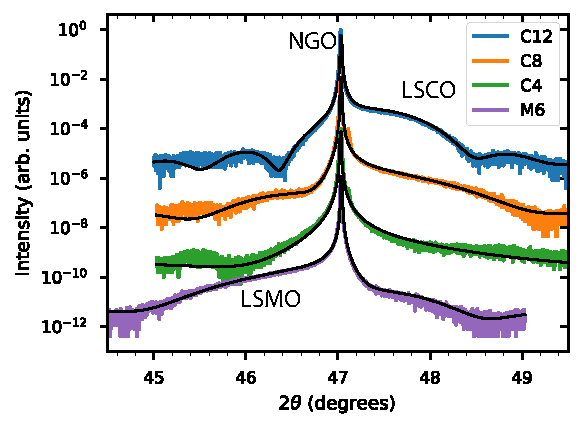
\includegraphics[width=.6\textwidth]{figures/results1/single_220.pdf}
    \caption{$\theta-2\theta$ scan about the NGO \hkl(2 2 0)$_o$ peak for single layer films C12, C8, C4, and M6}
    \label{fig:singlelayer_xrd}
\end{figure}
\begin{figure}[tb!]
    \centering
    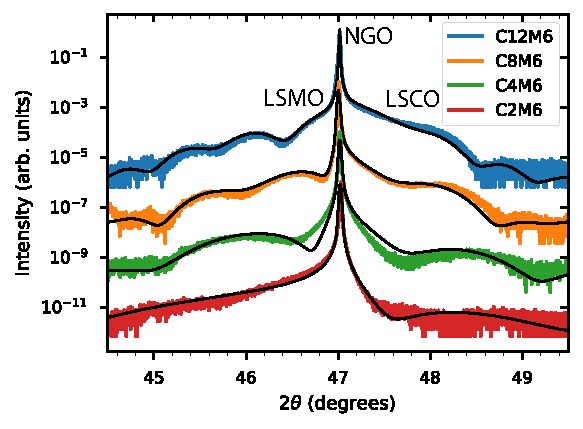
\includegraphics[width=.6\textwidth]{figures/results1/bilayer_220.pdf}
    \caption{$\theta-2\theta$ scan about the NGO \hkl(2 2 0)$_o$ peak for bilayer films C12M6, C8M6, C4M6, and C2M6}
    \label{fig:bilayer_xrd}
\end{figure}
\begin{table}[b!]
\centering
\caption{Structural parameters from xrayutilities fits to single layers C12, C8, C4, and M6. 3$\sigma$ confidence intervals reported in parenthesis.}
\label{tab:singlelayer_xrd}
\begin{tabular}{@{}lll@{}}
\toprule
Sample & $t$ (\si{nm}) & $c$ (\si{\angstrom}) \\ \midrule
C12 & 11.20(23) & 3.819(2) \\
C8 & 6.15(29) & 3.814(3) \\
C4 & 2.31(25) & 3.832(7) \\
M6 & 6.17(20) & 3.924(3)  \\
\bottomrule
\end{tabular}
\end{table}
\begin{table}[tb!]
\centering
\caption{Structural parameters from xrayutilities fits to LSMO / LSCO bilayers. 3$\sigma$ confidence intervals reported in parenthesis.}
\label{tab:bilayer_xrd}
\begin{tabular}{@{}lllllll@{}}
\toprule
& & \multicolumn{2}{c}{LSCO} & & \multicolumn{2}{c}{LSMO} \\
\cmidrule{3-4} \cmidrule{6-7}
Sample && $t$ (\si{nm}) & $c$ (\si{\angstrom}) && $t$ (\si{nm}) & c (\si{\angstrom})\\ \midrule
C12M6 && 9.94(25) & 3.815(2) && 5.29(18) & 3.908(4)\\
C8M6 && 6.18(26) & 3.801(3) && 6.21(14) & 3.909(3) \\
C4M6 && 3.30(43) & 3.840(1) && 5.01(11) & 3.902(1) \\
C2M6 && 0.50(13) & 3.813(32) && 4.51(6) & 3.924(2) \\
\bottomrule
\end{tabular}
\end{table}
Fits generated using a dynamical diffraction model, created with xrayutilities~\cite{Kriegner2013b}, are overlaid on the experimental data as black lines.  
For the fits, the NGO out-of-plane lattice parameter was fixed to \SI{3.864}{\angstrom} while the film thicknesses and lattice parameters were allowed to freely vary.  
The model used for XRD fits consists of a single layer for each material with a constant out-of-plane lattice parameter.  
A peak at \SI{45.5}{\degree} arises due to tungsten contamination of the copper x-ray tube, and is not captured by the XRD fits.  
Structural parameters derived from the single layer fits are given in Table~\ref{tab:singlelayer_xrd} while those from bilayer fits are in Table~\ref{tab:bilayer_xrd}.  
The reported errors correspond with a $3-\sigma$ confidence interval, with the typical error being within \SI{.003}{\angstrom} for the lattice parameter and \SI{.25}{\nm} for the layer thickness.  
For the single layer films, the LSCO lattice parameter is not sensitive to variation in LSCO film thickness.  
C4 has a slightly larger out-of-plane lattice parameter; however, the absence of any prominent features in the $\theta-2\theta$ scan for C4 suggests the out-of-plane lattice parameter derived from fits is not reliable.  
Poor fits to the diffuse scattering around the substrate peak for bilayer C4M6 also indicate that the model used is not completely accurate.  

$\theta-2\theta$ scans were also measured for samples C12, M6, and C12M6 at a SSRL beamline 7-2.  
Experimental data with fits are shown in Figure~\ref{fig:ssrl_xrd}, with structural parameters from the fits in Table~\ref{tab:ssrl_xrd}.  
The diffraction peak shapes are fit well for all samples, while thickness oscillations for sample C12M6 are not well fit on the high angle side of the main diffraction peak.  
\begin{figure}[tb]
    \centering
    \includegraphics[width=.6\textwidth]{figures/results1/ssrl_fits.pdf}
    \caption{$\theta-2\theta$ scans and fits for C12M6, C12, and M6, measured at SSRL BL 7-2}
    \label{fig:ssrl_xrd}
\end{figure}
\begin{table}[tb!]
\centering
\caption{Structural parameters from xrayutilities fits to BL 7-2 $\theta-2\theta$ scans.  3$\sigma$ confidence intervals reported in parenthesis.}
\label{tab:ssrl_xrd}
\begin{tabular}{@{}lllllll@{}}
\toprule
& & \multicolumn{2}{c}{LSCO} & & \multicolumn{2}{c}{LSMO} \\
\cmidrule{3-4} \cmidrule{6-7}
Sample && $t$ (\si{nm}) & $c$ (\si{\angstrom}) && $t$ (\si{nm}) & c (\si{\angstrom})\\ \midrule
C12M6 && 10.37(20) & 3.809(3) && 5.37(13) & 3.912(4)\\
C12 && 11.30(15) & 3.819(3) && - & - \\
M6 && - & - && 5.97(12) & 3.931(4) \\
\bottomrule
\end{tabular}
\end{table}
The higher dynamic range of synchrotron-based measurements results in the observation of significantly more thickness fringes compared with a lab-source and therefore the thickness values in Table~\ref{tab:ssrl_xrd} are considered to be more accurate compared with values derived from the lab-based diffractometer.  
Considering the uncertaity, the derived thicknesses and lattice parameters from both the synchrotron and lab-based diffractometer are in close agreement.  

There is a slight discrepancy between total film thicknesses derived from XRR fits and those from XRD fits, especially for the bilayer sample series.  
The total thickness for bilayers C12M6, C8M6, and C4M6 from lab-based XRD fits is \SI{10}{\percent} smaller than from XRR fits, and for bilayer C2M6 the difference is even more pronounced with a \SI{30}{\percent} difference between XRR and XRD derived thicknesses.  
When XRD data is fit, information about film thickness is derived by the diffracted peak shape.  
Thin films create broad diffraction peaks with low integrated peak intensity while thick films produce narrow peaks with high integrated peak intensity~\cite{Cullity1956}.  
Additional sources of peak broadening include the presence of any d-spacing variations within the film which can be caused by stoichiometry variations or relaxation.  
If d-spacing variations are present, a single layer model will account for additional broadness by altering the film thickness.  
Furthermore, XRD fits cannot account for the presence of any amorphous layers.  
Because XRR is insensitive to crystallographic information such as d-spacing variations or whether or not the film is crystalline or amorphous, there can be disagreement in XRR and XRD derived film thicknesses.  

\section{Reciprocal Space Maps}

Reciprocal space maps (RSM) were recorded about the NGO \hkl(3 3 2)$_o$ = \hkl(1 0 3)$_{pc}$ and \hkl(4 2 0)$_o$ = \hkl(0 1 3)$_{pc}$ peaks, which are rotated by \SI{90}{\degree} in $\phi$ from one another.  
Maps must be recorded at both orientations to confirm films are coherently strained along the two inequivalent in-plane directions of the orthorhombic NGO substrate.  
Because NGO substrates are orthorhombic, the out-of-plane position of the \hkl(1 0 3)$_{pc}$ and \hkl(0 1  3)$_{pc}$ peaks will be at different locations in reciprocal space~\cite{Vailionis2011}.  
RSMs for single layer C12 are shown in Figure~\ref{fig:c12_asym_rsm}.  
The film and substrate peaks occur at the same in-plane value indicating that the film is coherently strained to the substrate.  
\begin{figure}[b!]
    \centering
    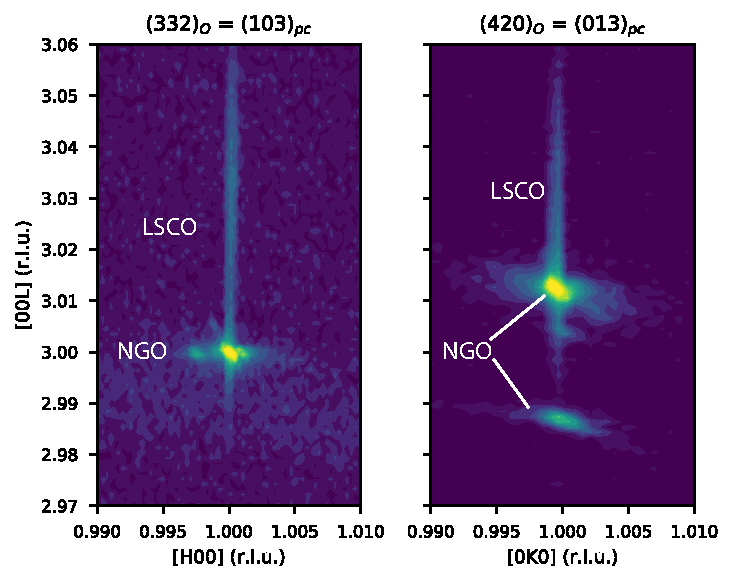
\includegraphics[width=.7\textwidth]{figures/results1/NA04_asym_rsms.pdf}
    \caption{C12 RSMs}
    \label{fig:c12_asym_rsm}
\end{figure}
RSMs for single layer C8 (Figure~\ref{fig:c8 rsm}), bilayer C12M6 (Figure~\ref{fig:c12m6_asym_rsm}), and bilayer C8M6 (Figure~\ref{fig:c8m6_rsm}) also confirm that these films are coherently strained.  
\begin{figure}[h!]
    \centering
    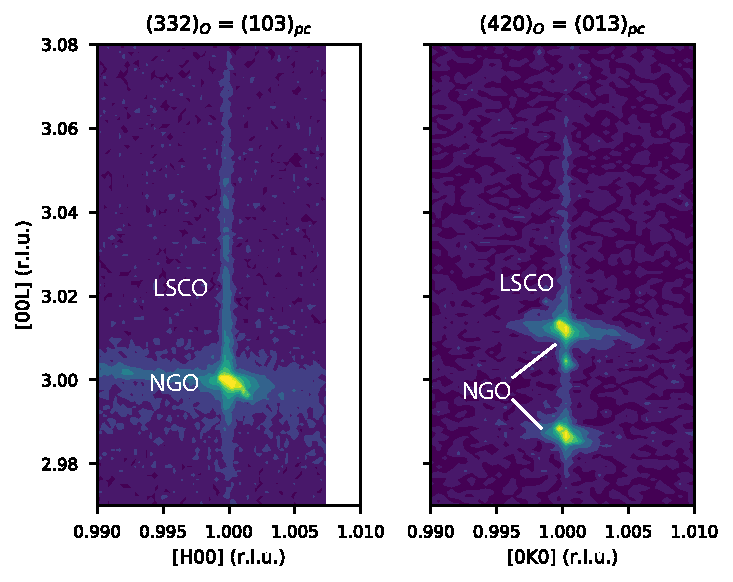
\includegraphics[width=.7\textwidth]{figures/results1/NA06_asym_rsms.pdf}
    \caption{C8 RSMs}
    \label{fig:c8 rsm}
\end{figure}
\begin{figure}[h!]
    \centering
    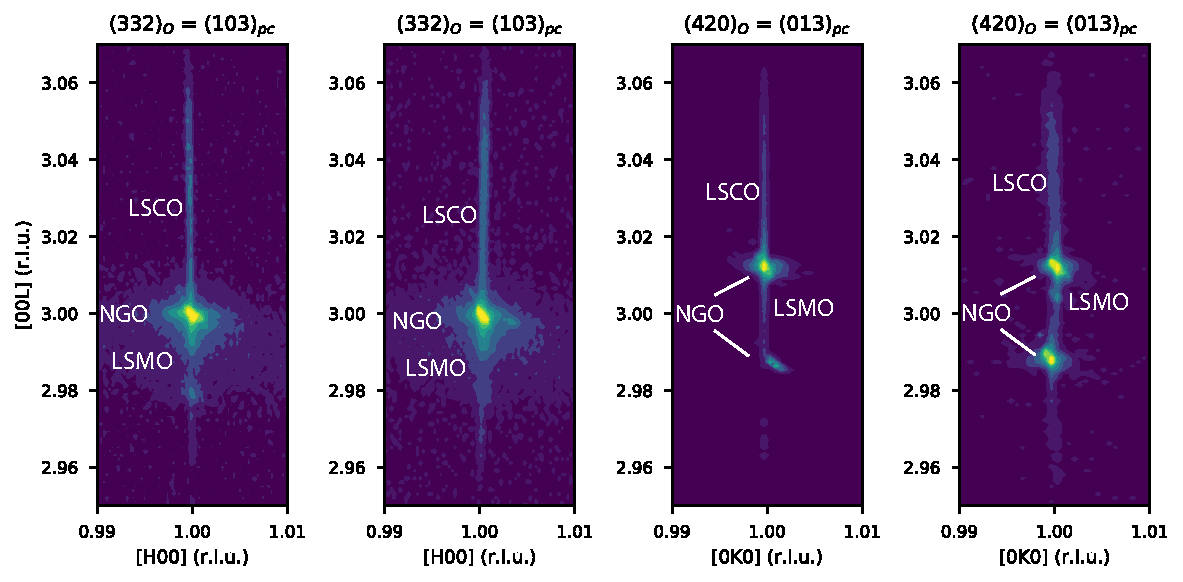
\includegraphics[width=\textwidth]{figures/results1/NA08_asym_rsms.pdf}
    \caption{C12M6 RSMs}
    \label{fig:c12m6_asym_rsm}
\end{figure}
\begin{figure}[h!]
    \centering
    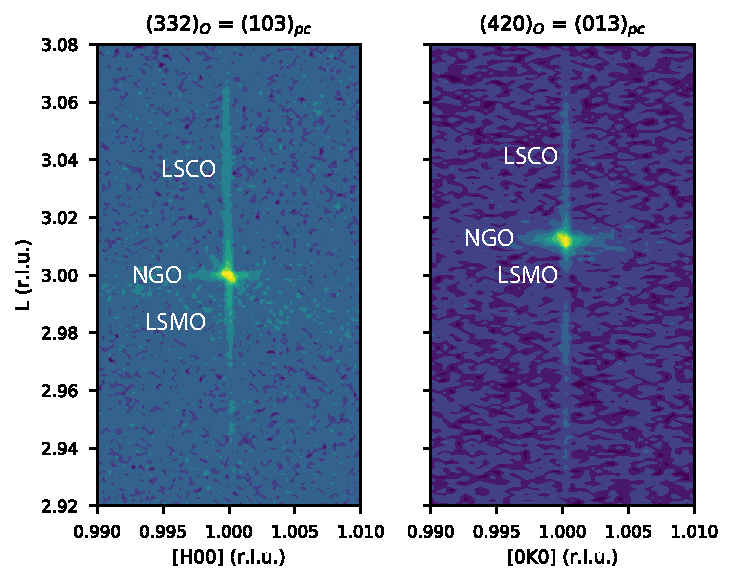
\includegraphics[width=.7\textwidth]{figures/results1/na09_asym_rsms.pdf}
    \caption{C8M6 RSMs}
    \label{fig:c8m6_rsm}
\end{figure}
The \hkl(4 2 0)$_o$ RSM shows two substrate peaks at different L positions for films C12, C8, and C12M6, while bilayer C8M6 only shows one substrate peak.  
This double substrate peak points to there being two structural domains within the substrate rotated \SI{180}{\degree} from one another.  
Substrate pieces are cut from a larger wafer, therefore certain substrate pieces may bisect both domains while others will only contain a single structural domain.  
RSMs about the \hkl(4 2 0)$_o$ peak are sensitive to the difference in the orthorhombic $a_o$ and $b_o$ directions and therefore the presence of rotated structural domains is only observable for this peak.  

A small tilt of approximately \SI{0.3}{\degree} between the LSCO film and substrate peak locations is present in the \hkl(3 3 2)$_o$ RSMs indicating that the film has bond angle deviation away from \SI{90}{\degree} along this direction.  
In Figure~\ref{fig:rsm_bond_angle}, a zoomed in image of the C12 \hkl(3 3 2)$_o$ RSM is shown making the bond angle deviation more clear. 
\begin{figure}[tb!]
    \centering
    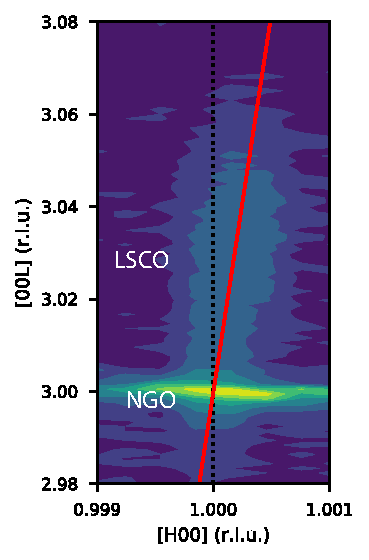
\includegraphics[width=.4\textwidth]{figures/results1/rsm_angle.pdf}
    \caption{C12 \hkl(3 3 2)$_{o}$ RSM zoomed in to emphasize the bond angle deviation from \SI{90}{\degree}}
    \label{fig:rsm_bond_angle}
\end{figure}
This deviation is only observed for \hkl(3 3 2)$_o$ RSMs meaning that this angle variation is only occurring for one of the bond angles resulting in a monoclinic unit cell for the growing LSCO and LSMO films on NGO substrates.  
The observed bond angle deviation has been reported for other perovskite films on orthorhombic substrates, such as \ce{SrRuO3} films on \ce{DyScO3} substrates~\cite{Vailionis2011}.   


\clearpage
\section{Diffraction from Half Order Peaks}
In the ideal perovskite structure, the B-O-B bond chains connecting each \ce{BO6} octahedra all make \SI{180}{\degree} angles leading to cubic symmetry.  
To accommodate ions of different sizes, as well as to accommodate interfacial strain, the \ce{BO6} octahedra can cooperatively rotate away from their ideal positions altering the overall symmetry of the structure.  
These octahedral rotations are classified by three angles about a pseudocubic set of axis, with $\alpha$ about the \hkl[1 0 0]$_{pc}$ direction, $\beta$ about the \hkl[0 1 0]$_{pc}$ direction, and $\gamma$ about the \hkl[0 0 1]$_{pc}$ direction, as depicted in Figure~\ref{fig:octahedra tilt angles}.  
\begin{figure}[b!]
    \centering
    \includegraphics[width=.4\textwidth]{figures/results1/may_tiltangles.png}
    \caption{Oxygen octahedral tilt angles about the three pseudocubic axes, from~\cite{May2010}.}
    \label{fig:octahedra tilt angles}
\end{figure}

Consider rotation by an arbitrary angle in the out-of-plane direction in one \ce{BO6} octahedra.  
In order to maintain B-O-B bond chain connectivity, the nearest neighbor \ce{BO6} octahedra must rotate in an opposite direction, as depicted in Figure~\ref{fig:oor double symm}.  
\begin{figure}[h]
    \centering
    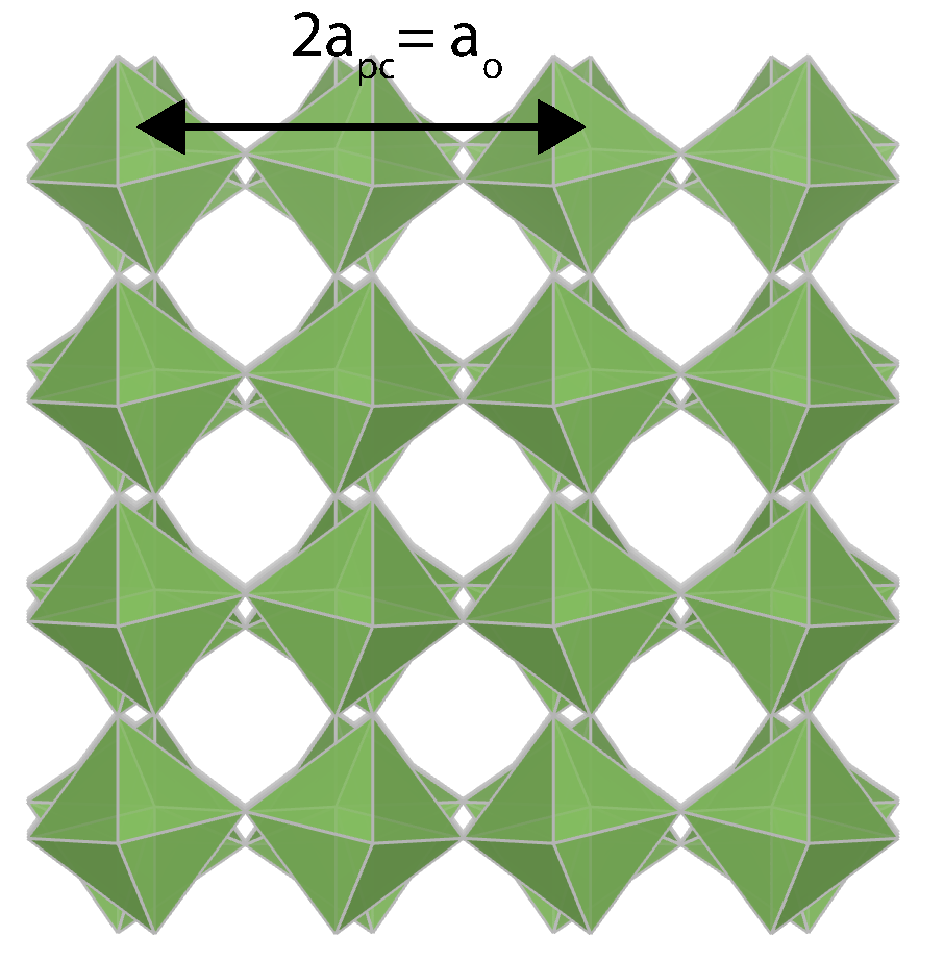
\includegraphics[width=.35\textwidth]{figures/results1/tilts_doubling.pdf}
    \caption{Doubling of the in-plane lattice parameter as a result of \ce{BO6} octahedral rotations around the out-of-plane direction}
    \label{fig:oor double symm}
\end{figure}
As a consequence of rotations about an out-of-plane axis, the material's in-plane lattice parameter has now doubled and the overall symmetry of the structure is altered.  
Octahedral rotations can be further classified as in-phase or out-of-phase.  
For out-of-phase rotations, the rotation direction about an axis changes from clockwise to counter clockwise in neighboring octahedra along the rotation axis while for in-phase rotations, the direction of rotation remains the same.  
Out-of-phase rotations therefore double the lattice parameter both parallel and perpendicular to the chosen rotation axis.  

Glazer outlined all of the possible octahedral rotation patterns for perovskites in two papers in the 1970s~\cite{Glazer1972,Glazer1975} and identified a total of 23 possible patterns.  
To classify these patterns, a three index notation was devised where each index corresponds with rotations about a particular axis with a superscript dictating in-phase versus out-of-phase rotations.  
For example, NGO takes on an $a^-b^+a^-$ octahedral rotation pattern.  
Rotations about the \hkl[1 0 0]$_{pc}$ and \hkl[0 0 1]$_{pc}$ axis are both out-of-phase, denoted by a $(-)$ superscript, and have the same rotation magnitude identified by the same letter, while rotations about the \hkl[0 1 0]$_{pc}$ axis are in-phase and have a different magnitude.  
Both LSCO and LSMO take on an $a^-a^-a^-$ tilt pattern in bulk with B-O-B bond angles of \SI{167}{\degree} and \SI{166.3}{\degree} respectively,  corresponding with average octahedral rotation angles of \SI{6}{\degree} and \SI{6.8}{\degree}~\cite{Caciuffo,Huijben2017}.  

Glazer's seminal work also outlines which rotation patterns lead to specific x-ray diffraction peaks.  
Recall that out-of-phase rotations change the lattice parameter in all three directions while in-phase rotations only change the lattice parameter in two directions.  
As a result, out-of-phase rotations create diffraction peaks with three half-order indices while peaks arising from in-phase rotations will have one integer index and three half-order indices.  
A diffraction peak \hkl(h k l) with all half order indices and $h \neq l$ is indicative of out-of-phase rotations about the $b$ axis.  
The complete set of rules is listed in Table~\ref{tab:halforder_rules}.  
\begin{table}[tb!]
\centering
\caption{Rules dictating the half order peaks observed for different types of octahedral rotations about the three principal axes, from~\cite{Glazer1975}}
\label{tab:halforder_rules}
\begin{tabular}{@{}cc@{}}
\toprule
Rotation & Peak Type \\ \midrule
$a^+$ & (h $\dfrac{\mathrm{k}}{2}$ $\dfrac{\mathrm{l}}{2}$),   $k\neq l$ \\\addlinespace
$b^+$ & ($\dfrac{\mathrm{h}}{2}$ k $\dfrac{\mathrm{l}}{2}$),   $h\neq l$ \\\addlinespace
$c^+$ & ($\dfrac{\mathrm{h}}{2}$ $\dfrac{\mathrm{k}}{2}$ l),   $h\neq k$ \\\addlinespace
$a^-$ & ($\dfrac{\mathrm{h}}{2}$ $\dfrac{\mathrm{k}}{2}$ $\dfrac{\mathrm{l}}{2}$),   $k\neq l$ \\\addlinespace
$b^-$ & ($\dfrac{\mathrm{h}}{2}$ $\dfrac{\mathrm{k}}{2}$ $\dfrac{\mathrm{l}}{2}$),   $h\neq l$ \\\addlinespace
$c^-$ & ($\dfrac{\mathrm{h}}{2}$ $\dfrac{\mathrm{k}}{2}$ $\dfrac{\mathrm{l}}{2}$),   $h\neq k$ \\\addlinespace
\bottomrule
\end{tabular}
\end{table}
With these rules in mind, a sequence of half order peaks can be selected and searched for as a way to determine a resultant octahedral tilt pattern.  
First, one of each of the in-phase rotation peaks must be identified to determine whether or not any of the octahedral rotations are in-phase.  
After the three in-phase rotation peaks have been searched for, a sequence of six out-of-phase peaks are searched for.  
Each of these peaks would correspond with two possible types of rotations and, along with the knowledge of any in-phase rotations, they can be used to rule out and deduce the resulting octahedral rotation pattern.  

A half order peak search was carried out on a \SI{15}{\nm} LSCO film on NGO substrate (C15), as well as bilayer C12M6 and single layers C12 and M6.  
A sequence of 15 peaks from sample C15, where either a substrate peak or both a film and substrate peak were observed, is shown in Figure~\ref{fig:15nm lsco half order}.  
No intensity was seen for either the film or substrate with an integer index in the $h$ or $l$ position (e.g. \hkl(0 \tfrac{3}{2} \tfrac{7}{2}) and \hkl(\tfrac{3}{2} \tfrac{7}{2} 0)), while only substrate peaks were observed when the $k$ index is at an integer value.  
This set of half order diffraction peaks confirms the expected NGO bulk octahedral pattern of $a^-b^+a^-$.  
No film peaks were observed when one of the peak indices was an integer meaning that the LSCO film is in a rotation pattern with all out-of-phase rotations, in agreement with earlier investigations of LSCO thin films~\cite{Biegalski2014}.  

A smaller subset of half order peaks was observed for single layers C12 and M6, and bilayer C12M6, shown in Figures~\ref{fig:c12 half order},~\ref{fig:m6 half order}, and~\ref{fig:c12m6 half order}.  
\begin{figure}[h!]
    \centering
    \includegraphics[width=\textwidth]{figures/results1/NA03_halforder_peaks.pdf}
    \caption{Sequence of half order peaks observed for C15}
    \label{fig:15nm lsco half order}
\end{figure}
\clearpage

\begin{figure}[h!]
    \centering
    \includegraphics[width=\textwidth]{figures/results1/C12_halforder.pdf}
    \caption{Sequence of half order peaks observed for single layer C12}
    \label{fig:c12 half order}
\end{figure}
\begin{figure}[h!]
    \centering
    \includegraphics[width=\textwidth]{figures/results1/M6_halforder.pdf}
    \caption{Sequence of half order peaks observed for single layer M6}
    \label{fig:m6 half order}
\end{figure}
\begin{figure}[h!]
    \centering
    \includegraphics[width=\textwidth]{figures/results1/C12M6_halforder.pdf}
    \caption{Sequence of half order peaks observed for bilayer C12M6}
    \label{fig:c12m6 half order}
\end{figure}
\clearpage

For both single layer C12 and bilayer C12M6, LSCO layer film peaks were observed only when all three peak indices are fractional confirming that the LSCO layer has all out-of-phase rotations.  
The observed rotation pattern for the LSCO film differs the substrate rotation pattern $a^-b^+a^-$ as well as the observed rotation pattern for $\ce{La_{0.5}Sr_{0.5}CoO3}$ thin films, $a^0b^-c^-$~\cite{Biegalski2014}.  
Some of the peaks, such as the $(\tfrac{3}{2} -\tfrac{1}{2} \tfrac{3}{2})$ were recorded in a low-resolution direction leading to the observed broadness of the substrate peak.  
No peaks from LSMO were observed for single layer M6 or bilayer C12M6, which is either due to no octahedral rotations in the LSMO layer, small octahedral rotation angles not producing a recognizable film peak, or the small LSMO film thickness producing a low signal intensity.  


\section{Quantifying Octahedral Rotations}
The octahedral rotation angles $\alpha$, $\beta$, and $\gamma$ can be experimentally determined by simulating the peak intensity of half order peaks following the procedure of May \textit{et al}~\cite{May2010}.  
A 2x2x2 perovskite super cell is constructed, only considering the 24 oxygen ion positions.  
The octahedra are then rotated by the given rotation angles, and the peak intensity is calculated using Equation~\ref{eq:peak intensity},
\begin{equation}
    I = I_0 \frac{1}{\sin (\eta)} \frac{1}{\sin(2 \Theta)} \left(\sum_{j=1}^4 D_j |F_{hkl}|^2\right)
    \label{eq:peak intensity}
\end{equation}
Where $1 / \sin(\eta)$ is a footprint correction term, $1 / \sin(2 \Theta)$ is the Lorentz polarization factor, $D_j$ is the domain fraction volume, and $F_{hkl}$ is the structure factor of the oxygen atoms calculated using Equation~\ref{eq:structure factor},
\begin{equation}
    F_{hkl} = f_{\ce{O^2-}} \sum_{n=1}^{24} \exp \left[2 \pi i \left(h u_n + k v_n + l w_n\right)\right]
    \label{eq:structure factor}
\end{equation}
where $f_{\ce{O^2-}}$ is the \ce{O^2-} form factor.  
The domain fraction term accounts for the fact that there are four possible rotation directions leading to the geometrically equivalent placement of oxygen atoms, one with all three octahedral tilt angles being positive and the other three having two positive angles and one negative angle.  
The intensity of half order peaks is determined by fitting the film and substrate peaks using a pseudo-Voigt function, and then integrating the area under the film peak.  
Intensity corrections are applied next, after which the dataset is fit for the three rotation angles.  

The outlined procedure was carried out for sample C15 which has the most comprehensive number  of half-order peak observations.  
Figure~\ref{fig:domain_peak} shows four half order peaks from the same family of planes that are used to obtain information about the domain fraction term $D_j$.  
\begin{figure}[tb!]
    \centering
    \includegraphics[width=.6\textwidth]{figures/results1/domain_peak.pdf}
    \caption{L-scans through a set of symmetrically equivalent half-order peaks}
    \label{fig:domain_peak}
\end{figure}
Peaks where the sample is rotated \SI{180}{\degree} from one another have similar shapes and intensities, while those rotated \SI{90}{\degree} from one another have different peak shapes and intensities.  
This observation is consistent with the slightly asymmetric strain state imposed by the orthorhombic NGO substrate, and suggest that there is an uneven population of the different rotational domains.  
Fitting the experimental intensity of a half order peak is simple when the film and substrate peak are separated; however, overlap between the two peaks results in inaccurate intensity values from the film peak.  
Because of this, only peaks with little to no overlap between film and substrate are used in the fitting.  
The list of peaks used for the fits is given in Table~\ref{tab:fit peak indices}.  
With this limited number of peaks, the domain fraction term $D_j$ cannot be fit, and instead fits were performed with the $D_j$ term fixed with either equal occupation for all domains, or equal population for two domains with the other having no population.  
The rotation patterns $a^0b^-c^-$, $a^-b^0c^-$, $a^-b^-c^0$, $a^-a^-c^-$, and $a^-b^-c^-$ were all simulated, and the best fit based on a $\chi^2$ goodness of fit was for a $a^-b^-c^-$ rotation pattern.  
The $\chi^2$ values for the other rotation patterns tested were approximately one order of magnitude greater than that for $a^-b^-c^-$.  
Results using either four or two equally populated domains are presented in Figures~\ref{fig:all_domain} and~\ref{fig:twodomain}.  
Because of the limited number of peaks used in the fitting, the domain fraction term is fixed during the fits.  
Using just two structural domains provides the best fit to the experimental dataset based on the lower $\chi^2$ value, with octahedral rotation angles of $\alpha = \SI{5.62}{\degree} \pm \SI{3.75}{\degree} $, $\beta = \SI{9.604}{\degree} \pm \SI{2.30}{\degree}$, and $\gamma = \SI{4.343}{\degree} \pm \SI{4.51}{\degree}$.  
The best fit values for angles $\alpha$ and $\gamma$ are slightly smaller than the bulk LSCO value of approximately $\SI{6}{\degree}$ while the angle $\beta$ is larger, although the significant amount of error associated with the calculated angles prevents a rigoruous comparions between bulk and thin film results.  
The large amount of error associated with the half order diffraction peaks arises for several different reasons.  
First, accurately extracting the intensity of a half order film peak in the immediate vicinity of the substrate peak is prone to a significant degree of error, and by investigating film peaks at higher scattering angles, where the film and substrate peak separation is higher, would be preferred.  
Furthermore, the intensity of certain half order diffraction peaks shows a strong dependence on specific octahedral rotation angles~\cite{Brahlek2017}.  
By analyzing these specific half order diffration peaks the error on half order rotation angles can be minimized.  
\begin{figure}[tb!]
    \centering
    \begin{subfigure}[t]{0.4\textwidth}
        \centering
        \includegraphics[width=\textwidth]{figures/results1/a-b-c-_all_domains.png}
        \caption{}
        \label{fig:all_domain}
    \end{subfigure}
    ~
    \begin{subfigure}[t]{0.4\textwidth}
        \centering
        \includegraphics[width=\textwidth]{figures/results1/a-b-c-_d3d4.png}
        \caption{}
        \label{fig:twodomain}
    \end{subfigure}
    \caption{Results from half order intensity fits using an $a^-b^-c^-$ rotation pattern.  $2\sigma$ error bars included on simulated dataset.  (a) Fits with four equally populated rotational domains.  (b) Fits with two equally populated rotational domains}
    \label{fig: half order fits}
\end{figure}

\begin{table}[tb!]
\centering
\caption{Peaks used for the fittings in Figure~\ref{fig: half order fits}}
\label{tab:fit peak indices}
\begin{tabular}{@{}cc@{}}
\toprule
Index & Peak \\ \midrule
0 & ($\dfrac{3}{2}$ $\dfrac{3}{2}$ $\dfrac{5}{2}$ )\\\addlinespace
1 & ($\dfrac{3}{2}$ -$\dfrac{1}{2}$ $\dfrac{5}{2}$ )\\\addlinespace
2 & ($\dfrac{3}{2}$ $\dfrac{1}{2}$ $\dfrac{5}{2}$ )\\\addlinespace
3 & ($\dfrac{3}{2}$ $\dfrac{1}{2}$ $\dfrac{7}{2}$ )\\\addlinespace
4 & ($\dfrac{5}{2}$ $\dfrac{1}{2}$ $\dfrac{7}{2}$ )\\\addlinespace
5 & ($\dfrac{5}{2}$ $\dfrac{1}{2}$ $\dfrac{3}{2}$ )\\\addlinespace
\bottomrule
\end{tabular}
\end{table}

\section{Conclusion}

Structural characterization of single layer films and LSMO / LSCO bilayers grown on NGO substrates confirms high quality film growth with experimental thicknesses in close agreement with the desired thickness.  
RSMs confirm that the films are coherently strained to the substrate with a slight distortion to one of the in-plane unit cell angles resulting in a monoclinic unit cell.  
Analysis of half-order diffraction peaks suggests that LSCO films have out-of-phase rotations about all three axes when grown both as a single layer film and as the first layer in a LSMO / LSCO bilayer.  
Best fits to the intensity of half-order peaks show that LSCO films have octahedral rotation angles of $\alpha = \SI{5.62}{\degree} \pm \SI{3.75}{\degree} $, $\beta = \SI{9.604}{\degree} \pm \SI{2.30}{\degree}$, and $\gamma = \SI{4.343}{\degree} \pm \SI{4.51}{\degree}$.  
